\section{System to Build} \label{sec:promise}

%P1 introduce the two components we want to build
\sysname's main components will include a container locator and a virtualized NIC.
The container locator can figure out where the location of the container is and
decide the most efficient way for two containers to talk with each other (e.g. 
via shared memory, rdma or dpdk).
And the virtualized NIC emulates the necessary underlying resource structures 
(e.g., send queue or receive queue of the NIC). In this way, the application will
be using the standardized APIs without be aware of the actual communication
mechanisms. The architecture of \sysname is shown in Figure~\ref{fig:system_modules}.

     \begin{figure}[ht]
     \centering 
     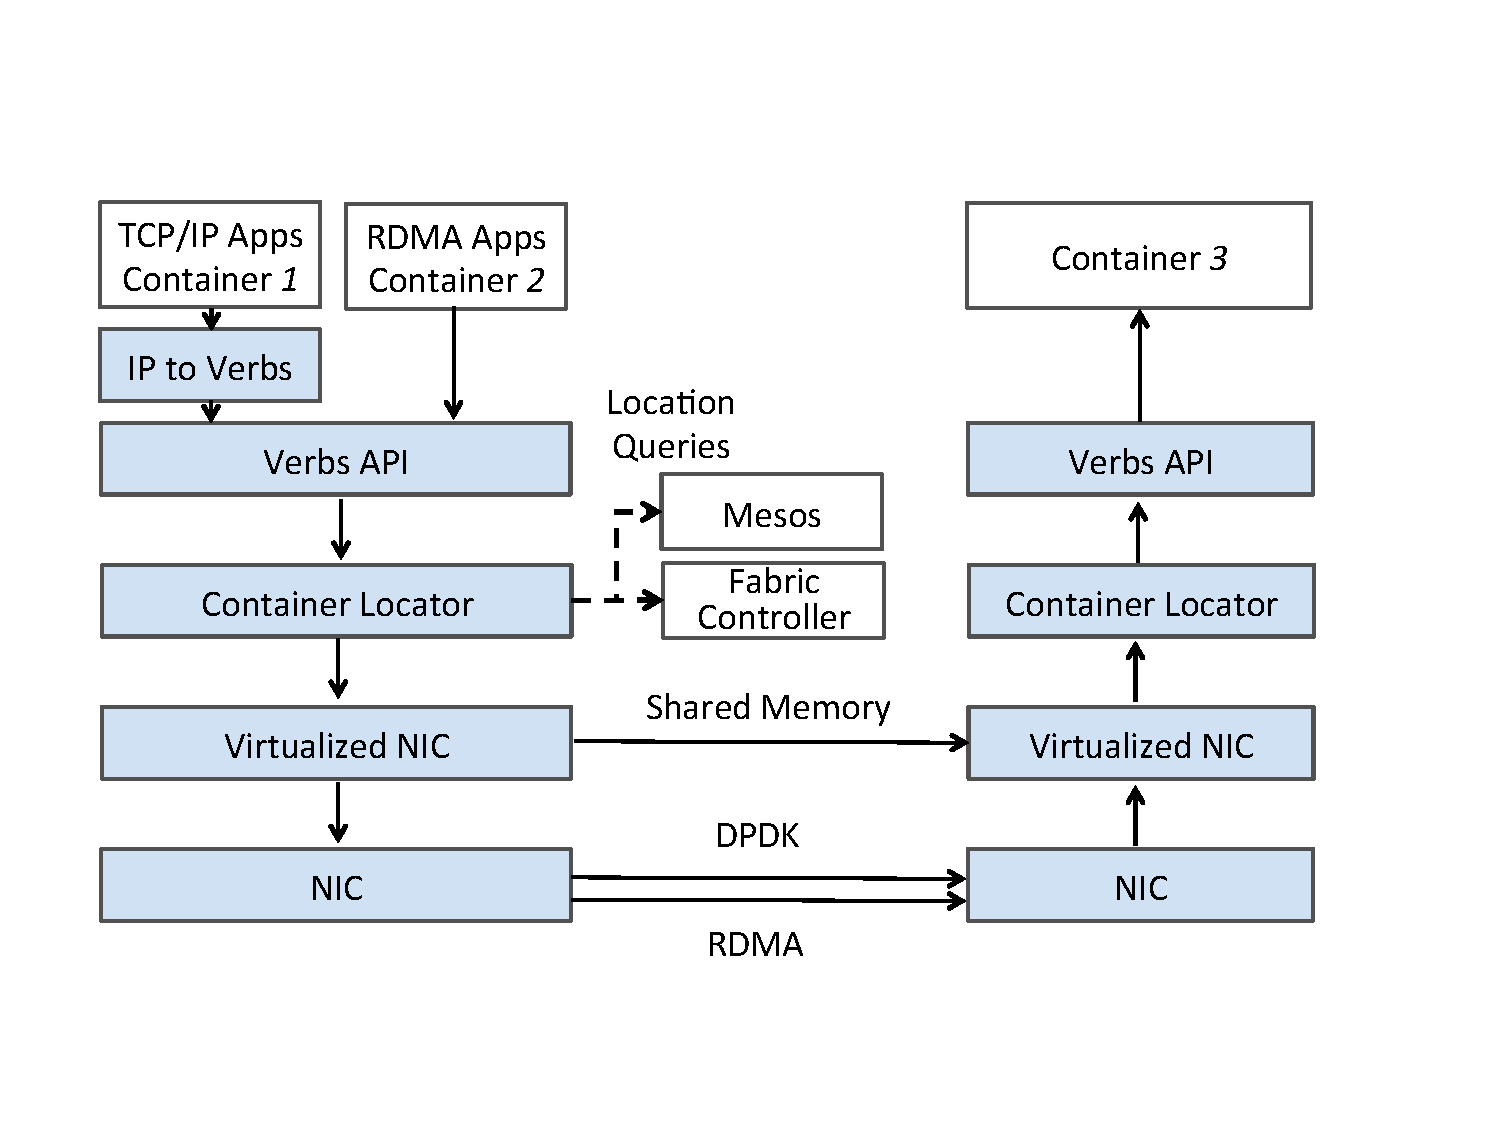
\includegraphics[width=0.5\textwidth]{figures/system/system_modules.pdf}      
     \label{fig:system_modules}
     \caption{The system architecture of \sysname.} 
     \end{figure}

\subsection{Container Locator}
The Container Locator is a logic module we will add inside the communication
library of a container's application. For example, if the application is a RDMA application,
the Container Locator will be inside library \texttt{libibverbs}. 

     \begin{figure}[ht]
     \centering 
     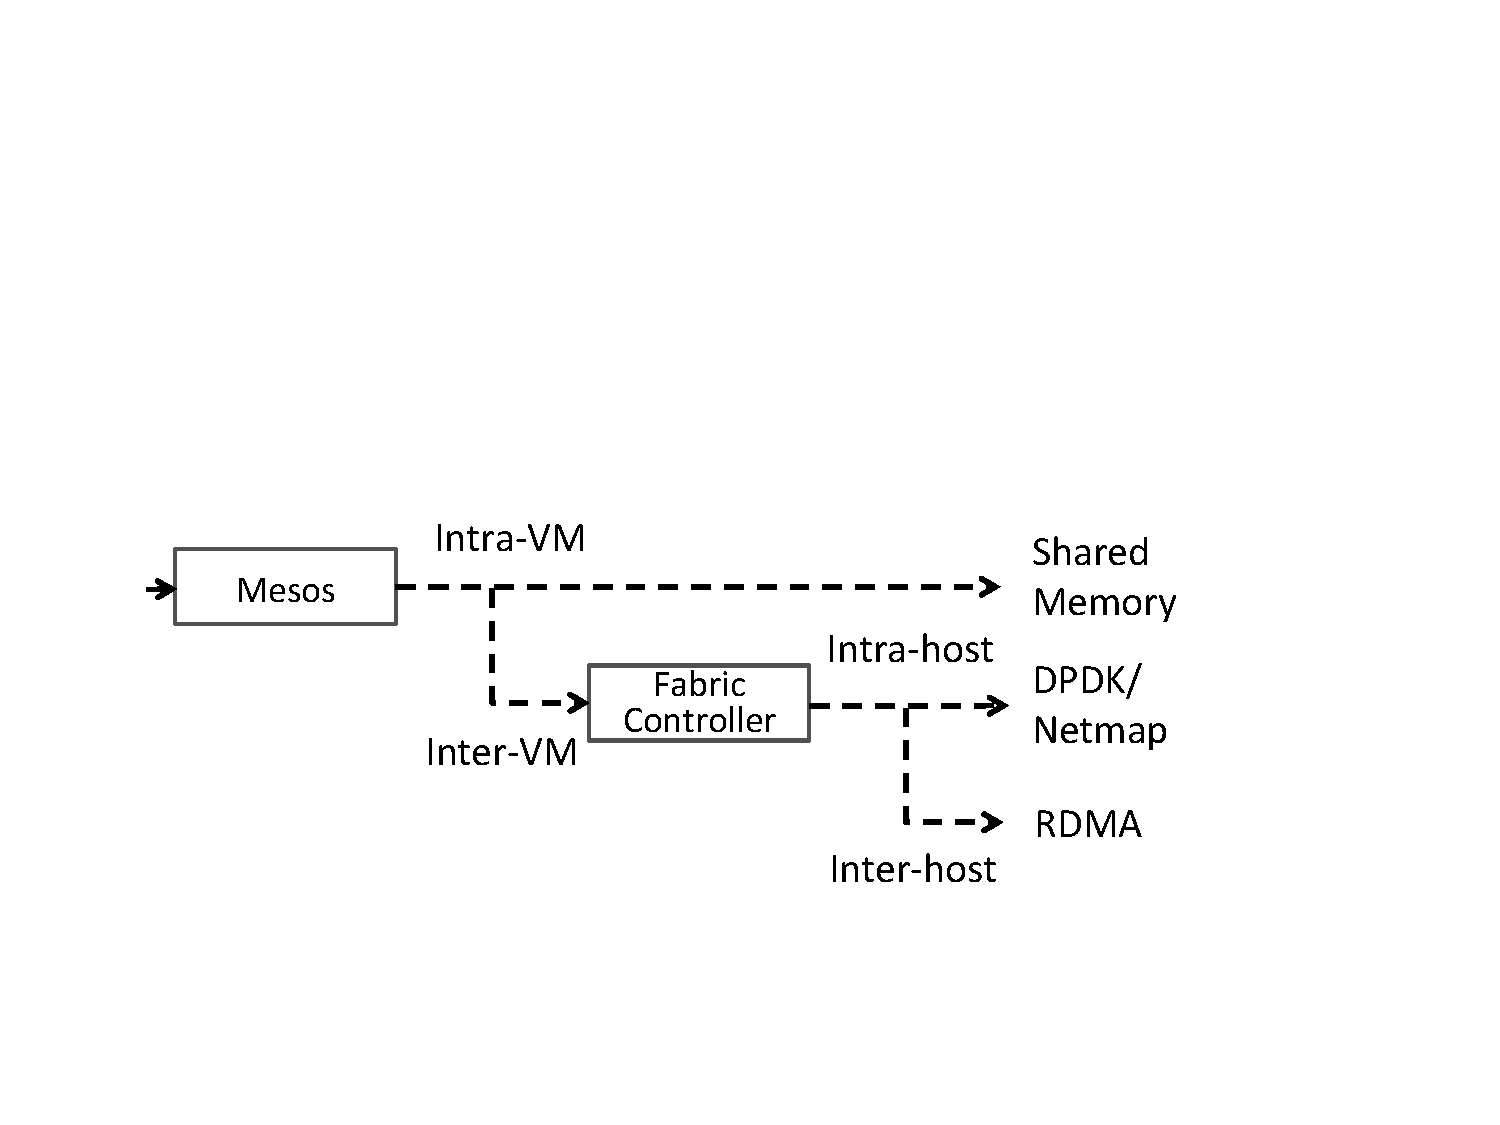
\includegraphics[width=0.45\textwidth]{figures/system/system_locator.pdf}      
     \label{fig:system_locator}
     \caption{The logic flow of Container Locator.} 
     \end{figure}

The Container Locator send queries to Mesos (resource manager) and the cloud's Fabric Controller to locate
the sender/receiver containers and decide the most efficient way they talk with each other.
The logic flow of this process is as shown in Figure~\ref{fig:system_locator}.
For example, given a send request, the Container Locator will query Mesos to figure out if the 
sender/receiver containers are intra-VM or inter-VM. 
For intra-VM containers, the Container Locator will raise a flag to notify the virtualized NIC to
send the data via shared memory.
For inter-VM containers, the Container Locator will then quire if the two containers are intra-host
or inter-host.
If the containers are inter-VM but intra-host, Container Locator will tell the virtualized NIC to send
the data via fast data pass across VMs in the same machine, such as NetVM\cite{} or netmaps\cite{}.
Or if the containers are inter-host, RDMA would be the most efficient way to perform the data transfer.

\tianlong{There should be some design decisions to support the above logic in design section.}

%We are going to add a logic module called Container Locator inside the application's
%library for communication. For example, the  

\subsection{Virtualized NIC}
The virtualized NIC acts as a transparent layer between the application and the underlying network structure, dynamically choosing the best communication mechanism, while maintaining compatibility with currently written applications.

The decision of which mechanism to chose is based on the hardware capabilities of the hosts and the physical placement of the containers, while aiming for minimal CPU overhead and high throughput. This decision and switching between communication mechanism is done completely transparent from application.

For intra-host communication, virtualized NIC will use shared memory communication inducing minimal pressure on the CPU while reaching high throughput (~ memory bandwidth). For inter-host communication, the virtualized NIC will prioritize RDMA communication when supported by the underlying hardware. Otherwise, it will use TCP/IP communication. 


